\tikzstyle{state}=[circle,draw=blue!50,fill=blue!20,thick,inner sep=0pt,minimum size=6mm]

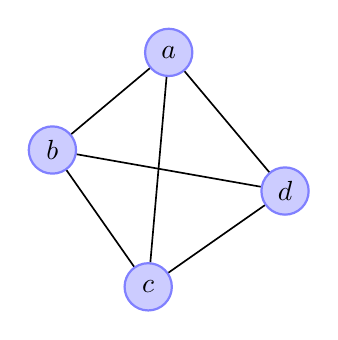
\begin{tikzpicture}[scale=1.5,node distance=3cm,semithick,bend angle=45,minimum size=0.1cm,draw,auto]
\node[state]   (a) at  (90:1) {$a$};
\node[state]   (b) at (170:1) {$b$};
\node[state]   (c) at (260:1) {$c$};
\node[state]   (d) at (350:1) {$d$};
\path
(a) edge (b)
    edge (c)   
    edge (d)
(b) edge (c)
    edge (d)
(c) edge (d);             
\end{tikzpicture}